\chapter{Analyse}\label{ch:analyse}

Bevor auf Grundlage der architekturellen Ideen aus \Cref{ch:grundlagen} ein konkretes Lösungskonzept entwickelt werden konnte, musste die bestehende App zunächst analysiert werden. Diese auf den Entwicklungsprozess vorbereitenden, analytischen Aspekte sollen in diesem Kapitel erörtert werden, um im nächsten Kapitel die konkreten Implementationskonzepte vorzustellen.

\section{Ermittlung einer Dialoglandkarte}

Zu Beginn der Analyse wurde die bestehende iOS App getestet, um alle möglichen Navigationswege und Dialoge zu sammeln und innerhalb einer Übersicht zu betrachten.

\begin{figure}[H]
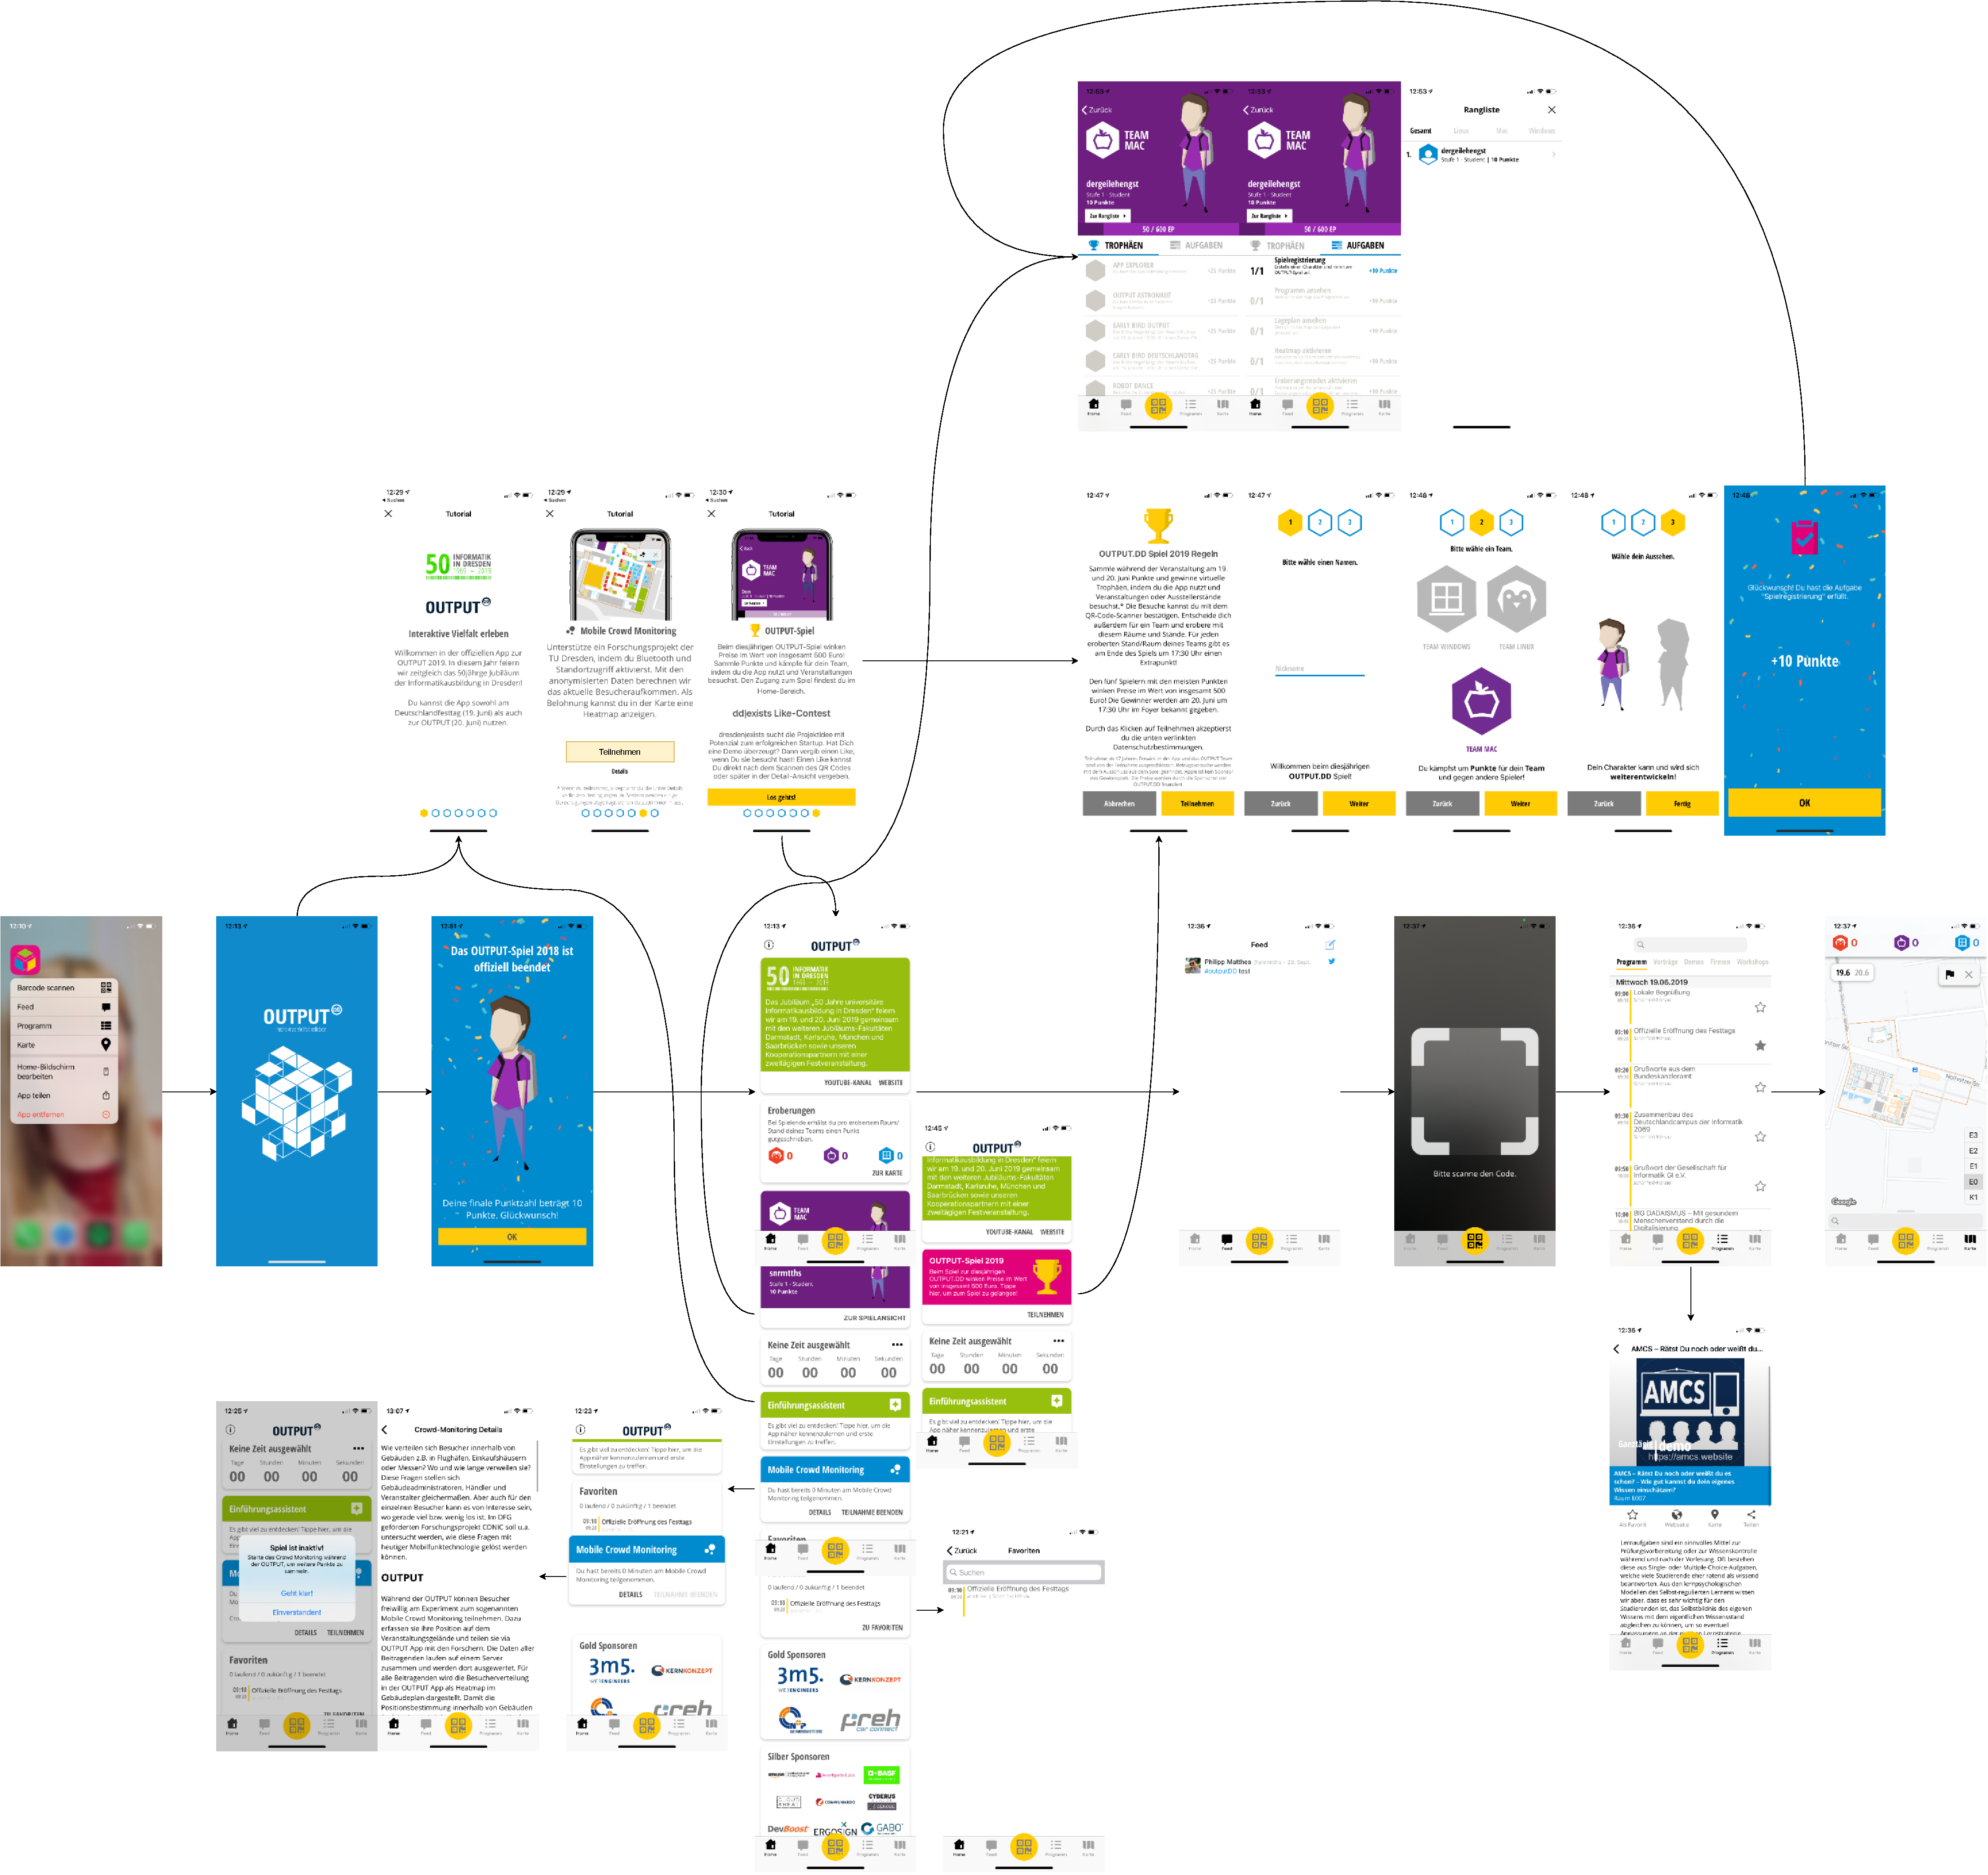
\includegraphics[width=\linewidth, bb=0 0 2123 2002]{mindmap.pdf}
\caption{Die erstellte Dialoglandkarte zur bestehenden Version der iOS App zeigt die Navigationswege innerhalb der App, sowie die genutzten UI-Elemente.}\label{fig:mindmap}
\end{figure}

Die in \Cref{fig:mindmap} gezeigte Dialoglandkarte suggeriert bereits die verschiedenen Gruppierungen von Ansichten, welche wir später zur Erstellung von neuen Packages heranziehen konnten. Zu sehen ist beispielsweise, dass die Spiel-Ansichten, der Einführungsassistent, oder bspw. auch die Kalender-Ansicht bereits gut voneinander separierbar sind. Die aufgezeichneten Navigationspfeile zwischen den Ansichten konnten genutzt werden, um die Datenflüsse hierbei vor der Erstellung des Konzeptes besser zu verstehen und die jeweils hierfür am Besten geeigneten Patterns zu finden.

\section{Struktur des Couchbase-Datenbank-Frameworks}

Die Persistierung der Applikationen kann über verschiedene Frameworks geschehen, iOS bietet standardmäßig bereits eine sehr rudimentäre Persitenzschnittstelle unter \texttt{UserDefaults}, auf Android analog hierzu \texttt{SharedPreferences}. Da jedoch nicht nur eine größere Anzahl an Daten persistiert werden müssen (Sponsoren, Spieldaten, Kalenderereignisse, Heatmap uvm.), sondern diese auch mit einem Server-Backend nach dem Offline-First-Prinzip synchronisiert werden sollen, kommen nur wenige fortgeschrittene Persistenz-Frameworks in Frage. Ehemals nutzten die Apps eine Realm-Datenbank, welche wegen externer Konditionen jedoch nicht mehr in Frage kam. Daher wurde ein Couchbase-Framework erstellt, inklusive eines Server-Backend-Systems, welches einen Synchronisationsservice und unter anderem auch einen Registrationsservice umfasst.

\begin{figure}[H]
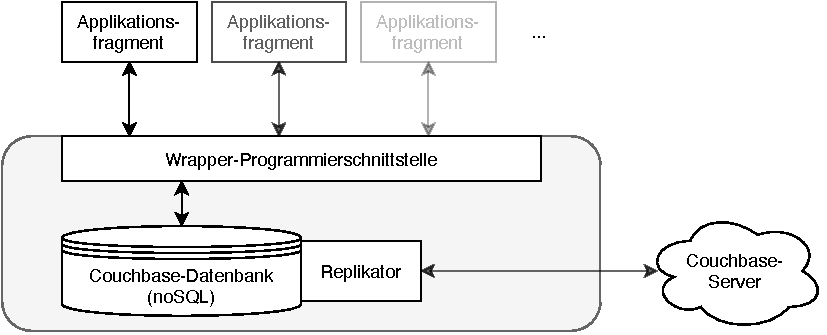
\includegraphics[width=\linewidth, bb=0 0 396 161]{wrapper.pdf}
\caption{Eine Übersicht über das zu integrierende Couchbase-Framework. Über eine abstrahierende Wrapper-Programmierschnittstelle wird auf die Datenbank zugegriffen.}\label{fig:wrapper}
\end{figure}

Die Metastruktur des Frameworks ist in \Cref{fig:wrapper} gezeigt. Um die Nutzung von Couchbase zu vereinfachen, wurde das Framework in eine abstrahierende Wrapper-Programmierschnittstelle eingebunden, welche die wichtigsten CRUD-Operationen, On-Change-Listener und auch die Synchronisationskomponente (Replikator) bereitstellt.

\begin{figure}[H]
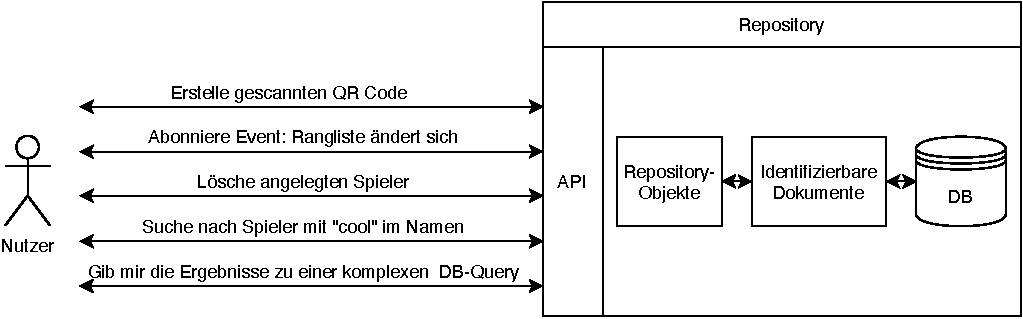
\includegraphics[width=\linewidth, bb=0 0 491 153]{repository.pdf}
\caption{Das Couchbase-Framework kapselt die Datenmodelle in voneinander separierte Repositories, auf denen unter anderem grundlegende CRUD-Operationen möglich sind.}\label{fig:repository}
\end{figure}

\Cref{fig:repository} illustriert, wie die Datenmodelle der Applikation geschrieben und gelesen werden können. Die Repository-Schnittstelle des jeweiligen Datenmodells bietet die dazugehörigen Funktionalitäten an.

\begin{figure}[H]
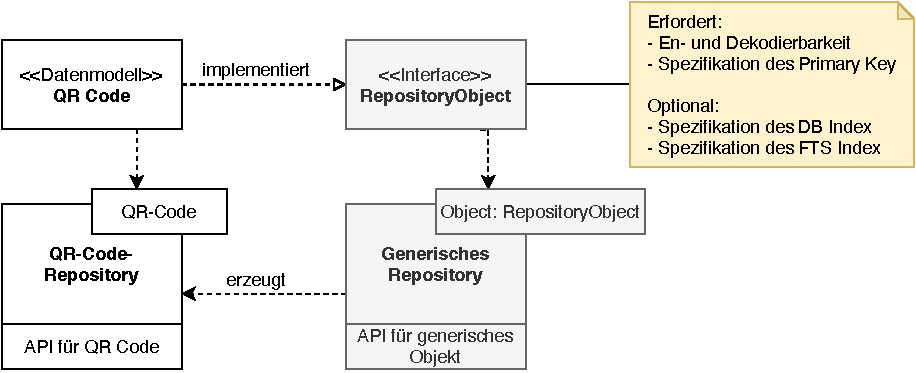
\includegraphics[width=\linewidth, bb=0 0 439 179]{generics.pdf}
\caption{Die Repository-Schnittstelle wird generisch durch das Datenmodell und das dazugehörige Repository erzeugt. Der Änderungsaufwand bei einer Änderung des Datenmodells ist somit sehr gering und neue Datenmodelle können ohne größeren Aufwand hinzugefügt werden.}\label{fig:generics}
\end{figure}

Wie in \Cref{fig:generics} gezeigt, werden die Repositories vom Framework generisch inferiert und anschließend in Form von standardisierte Schnittstellen bereitgestellt. Die diesen Schnittstellen zugrunde liegenden Datenbankabfragen müssen somit in der App nicht implementiert werden. Gleichzeitig kann das Datenbank-Backend bei Fortbestehen der Schnittstellen auch im Hintergrund ausgetauscht werden, ohne Änderungen in der App zu bedingen.

\section{Top-Level-Architektur und Muss-Kriterien}

Auf Grundlage der erstellten Dialoglandkarte sowie der bekannten Datenbankstruktur des Couchbase-Frameworks wurde ein Top-Level-Architektur-Modell (TLA) erstellt, um die Applikation in voneinander weitestgehend unabhängige Teilbereiche zu separieren.

\begin{figure}[H]
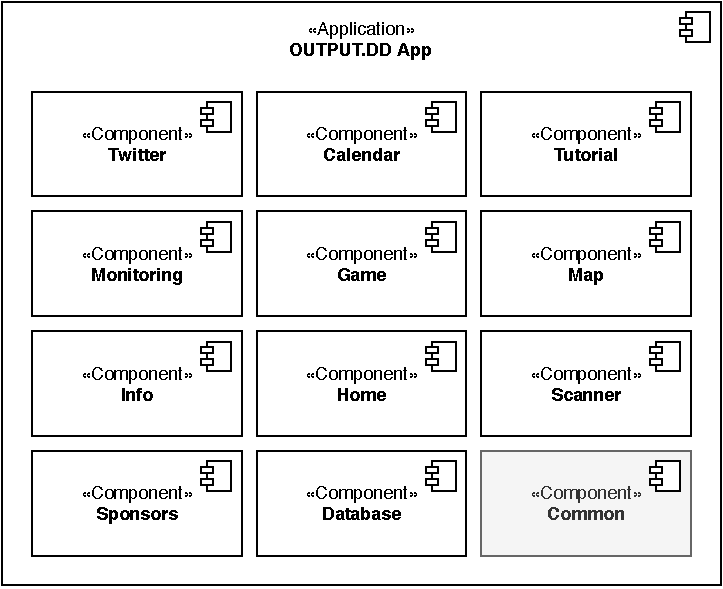
\includegraphics[width=\linewidth, bb=0 0 347 282]{tla.pdf}
\caption{Die TLA der Applikation im Überblick.}\label{fig:tla}
\end{figure}

Wie in \Cref{fig:tla} zu sehen, wurde die Applikation in 12 Komponenten unterteilt. Im folgenden werden die zu diesen Komponenten gehörenden Muss-Kriterien erläutert:

\begin{itemize}
    \item \textbf{Twitter} stellt alle Feed-Funktionalitäten bereit, inklusive der Feed-Ansicht und der Möglichkeit, neue Tweets zu erstellen.
    \item \textbf{Calendar} realisiert die Kalender-Ansicht des Veranstaltungsplans, inklusive der Detailansichten zu den jeweiligen Ereignissen, einer Möglichkeit, Ereignisse zu favorisieren, sowie nach bestimmten Ereigniskategorien zu filtern und zu suchen.
    \item \textbf{Tutorial} stellt alle Funktionalitäten und Ansichten des Einführungsassistenten bereit, welcher die wesentlichsten Bestandteile der App kurz erläutert.
    \item \textbf{Monitoring} kapselt die Crowd-Monitoring-Funktionalitäten des externen Crowd-Monitoring-Frameworks, sowie die Ansichten, die zur Erklärung und Steuerung dessen notwendig sind.
    \item \textbf{Game} ist die funktionell mächtigste Komponente, da sie alle Ansichten und Funktionalitäten der Gamification beinhaltet, darunter die Spielerregistrierung, die Trophäen- und Errungenschaften-Ansichten, die Fortschrittsansicht, die Rangliste sowie die Eroberungs-Ansicht.
    \item \textbf{Map} beinhaltet die Kartenansichten, darunter die Möglichkeiten der Auswahl bestimmter Etagen und Ansichtsoptionen wie die aktuellen Eroberungen oder die Anzeige des Besucheraufkommens über die Heatmap.
    \item \textbf{Info} stellt wichtige informative Ansichten bereit, darunter die Danksagungen und Lizenzen, aber auch Link-Ansichten zu Datenschutzerklärung und Impressum.
    \item \textbf{Home} dient als Verbinder zwischen verschiedenen Ansichten durch die Bereitstellung einer Home-Ansicht, auf der verschiedene Teilansichten und Links anderer Komponenten gezeigt werden.
    \item \textbf{Scanner} realisiert die QR-Code-Scanner-Funktionalitäten, die benötigt werden, um Errungenschaften für das OUTPUT-Spiel freizuschalten.
    \item \textbf{Sponsors} ist verantwortlich für die Bereitstellung von Ansichten zur Anzeige von Sponsoren in der Home-Ansicht.
    \item \textbf{Database} stellt die zum Couchbase-Framework ergänzend benötigten Ansichten und Schnittstellen bereit.
    \item \textbf{Common} stellt Komponenten und Erweiterungen bereit, die in der gesamten Applikation benötigt werden, beispielsweise eine modulare Card-Ansicht, die sich im UI (siehe Dialoglandkarte) häufig wiederfindet.
\end{itemize}

Diese TLA soll nachfolgend im Rahmen verschiedener Konzepte verfeinert und implementiert werden.
